\chapter{Sistema de control de temperatura}
\label{cap: control_temperatura}

Este capítulo describe el desarrollo de un sistema de calentamiento y control de temperatura para la plataforma de impresión. Esta plataforma de impresión figura como una sección más de la estación \acrshort{NPAM}, al igual que el extrusor y el manipulador robótico UR. 

El desarrollo del sistema de regulación automática de temperatura se ha hecho en colaboración con Irene Rodríguez Gramún. Se trata de una alumna cuyo trabajo se enfoca en el diseño y validación del regulador de temperatura desde una perspectiva electrónica y de diseño de producto, con tareas como  la concepción de un equipo protector de encapsulamiento y el conexionado del circuito integrado desarrollado a propósito para este equipo. Su aportación a esta fase del proyecto se especifica en las próximas líneas.

El capítulo inicia con una introducción al problema en la que se definirán los valores de mayor interés y las necesidades que se deben cubrir entre la plataforma de impresión y el resto de la estación. Posteriormente se describe la metodología seguida y los hitos en los que se ha divido; así como la coordinación empleada con otros participantes. Como punto final al capítulo se realiza una revisión de los resultados obtenidos, indicando las ventajas más relevantes del sistema y proponiendo algunas mejoras de cara a futuros proyectos.

El código descrito en este capítulo se encuentra en dos bloques diferentes: la implementación con ROS2 para las comunicaciones con el resto de la estación robotizada y el código del microcontrolador empleado como dispositivo regulador. El primer bloque está disponible en el repositorio Git del proyecto\footnote{Disponible en el direccionamiento: \textit{./workspace/ros\_ur\_driver/src/build\_platform}}\cite{repo_github_TFM_MiguelLerinAlonso} mientras que el segundo se ubica en dos posibles ubicaciones, la correspondiente al repositorio de este proyecto\footnote{Disponible en el direccionamiento: \textit{./control\_unit}}  y el repositorio especializado desarrollado por Irene Rodríguez\cite{repo_github_Irene_Rodriguez}.

\section{Introducción al problema}
Actualmente numerosos equipos de fabricación aditiva tipo \acrshort{MEX} integran la posibilidad de calentar la plataforma de impresión para favorecer la correcta deposición al mismo tiempo que se da un proceso de curado del material simultáneo. La responsabilidad de gestionar las variables asociadas a esta tarea -como por ejemplo el flujo de calor necesario, la temperatura media del sistema o electrónica de potencia necesaria- suele estar a cargo un microcontrolador diseñado expresamente para el equipo utilizado, de modo que raras ocasiones existe la posibilidad de intercambiar la cama de impresión.

Los sistemas robotizados que utilizan geometrías de piezas complejas ven prácticamente obligatoria la integración este tipo de sistemas para compensar nuevas variables relacionadas con la naturaleza de la plataforma de impresión. Tomando como referencia un sistema robotizado \acrshort{NPAM} como el de este proyecto, se observa que a las variables antes mencionadas se añade proporcionar una adherencia adecuada para el material depositado o resistir las inercias ocurridas durante el movimiento del manipulador.

La estación de fabricación con la que se trabaja en este proyecto se caracteriza por disponer una plataforma móvil acoplada al final de la cadena cinemática del cobot. Por su parte otros elementos como el sensor de distancia láser y el extrusor permanecen fijos en el espacio. Este enfoque se adopta con la intención de poder separar la plataforma de impresión del resto de elementos de la estación y poder cambiarla por otra distinta según necesidades. 

\section{Metodología}
El enfoque de diseño adoptado busca desacoplar la plataforma de impresión todo lo posible del resto la estación. Para ello se opta por dividir la plataforma en dos bloque funcionales fácilmente intercambiables: la cama de impresión desarrollada por Iñaki Echepare \cite{TFM_IñakiEchepare} y una unidad de control programable que regule la temperatura de la cama y comunique el estado de la cama al computador central de la estación. 

La Figura \ref{fig:arquitectura plataforma impresión} se utiliza para ilustrar esquemáticamente la arquitectura de control implementada en el sistema, siguiendo un enfoque de cliente-servidor. En ella también se definen los mensajes con los que se interactuará: lectura de temperatura, acción de control y comunicaciones con la estación de fabricación (estado de plataforma y arranque de unidad de control).

\begin{figure}[h!]
    \centering
    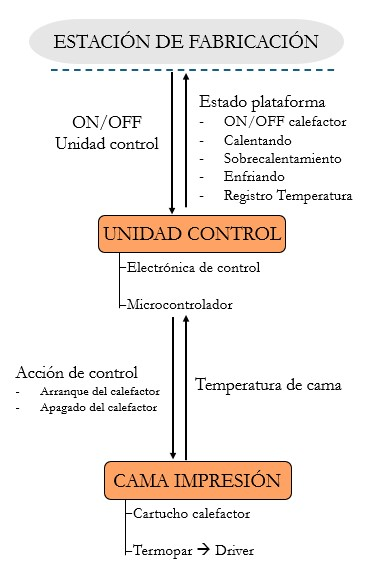
\includegraphics[scale=0.5]{figuras/arquitectura plataforma impresion.jpg}
    \caption{Arquitectura de control de plataforma de impresión}
    \label{fig:arquitectura plataforma impresión}
\end{figure}

\subsection{Lectura de temperatura}
Para el calentamiento de la superficie exterior de la cama de impresión se recurre a un cartucho calefactor introducido en su interior, a lo largo de su eje longitudinal.La lectura de su temperatura se realiza a través de un termopar introducido en el interior de la cama de impresión de forma adyacente. 

El modelo de termopar empleado es tipo K RS PRO \cite{RS_Online_Termopar_2024} y puede registrar un rango de temperaturas de -50 a +250 ºC con una precisión de $\pm$1.5 ºC. Por su parte, el rango de trabajo de la unidad de control empleada oscila entre los 0 y 5 V, lo que resulta insuficiente para efectuar una medida dependiendo únicamente de la conexión directa entre ambos elementos. Por este motivo se decide introducir una etapa intermedia de conversión de tensión mediante un amplificador de instrumentación. 

Ante el reducido precio de estos componentes y su facilidad de uso, se opta por adquirir un driver comercial especializado en la lectura de estos sensores\cite{manual_termopar_driver_max6675}, con una constante de conversión de 41 $\mu$V/ºC. La Figura \ref{fig:amplificador termopar} muestra el esquema eléctrico del amplificador de instrumentación comercial empleado.

\begin{figure}[h!]
    \centering
    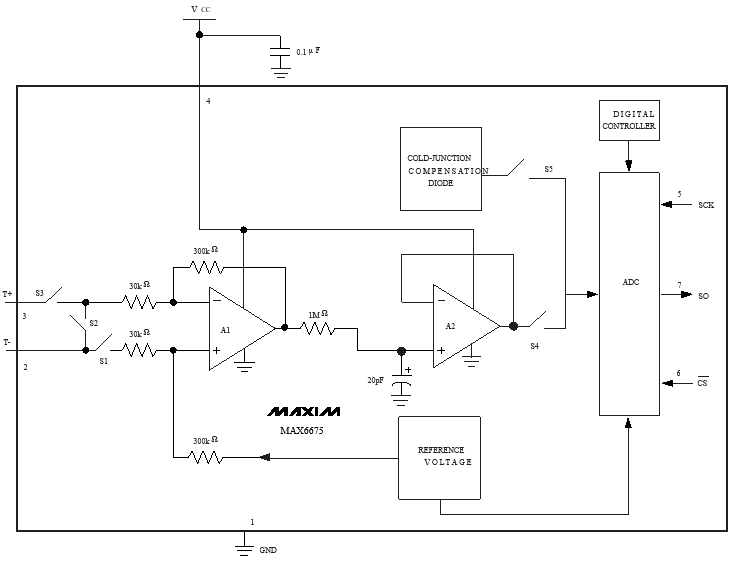
\includegraphics[scale=0.25]{figuras/amplificador termopar.png}
    \caption{Amplificador de instrumentación para el termopar\cite{manual_termopar_driver_max6675}}
    \label{fig:amplificador termopar}
\end{figure}

Con la versión previa del sistema de sensorizado construida se procede al desarrollo de un código de validación escrito en C/C++ para favorecer la interoperabilidad entre diferentes microcontroladores.

\subsection{Acción de control}
La alimentación del cartucho calefactor se realiza a través de un circuito de potencia conectado directamente a la red eléctrica del laboratorio (230 V AC y 50 Hz). 

Se decide dividir el circuito en dos etapas de control diferenciadas: una primera de control estático que se gestiona de forma manual por el propio operario de la estación, y otra situada aguas abajo de control dinámico accionado automáticamente por la unidad de control de la plataforma de impresión. 

El esquema eléctrico del sistema de regulación se aprecia en la Figura \ref{fig: Esquema eléctrico regulador de temperatura}, en ella se ha utilizado el simulador LTSpice \cite{LTSpiceSimulator} para validar el modelo funcionamiento del sistema. De derecha a izquierda se identifica la energía proveniente de la red eléctrica española con una tensión alterna de 325 V de valor pico a una frecuencia de trabajo de 50 Hz. Aguas abajo se ubica la etapa de control estático a través del modelo linealizado del potenciómetro empleado. Posteriormente se sitúa la etapa de control dinámico, representado por un circuito adyacente que modela la salida de un pin digital del microcontrolador empleado para la unidad de control y el relé responsable del accionamiento. Finalmente se cierra el circuito con la resistencia eléctrica representante del cartucho calefactor.

\begin{figure}[h!]
    \centering
    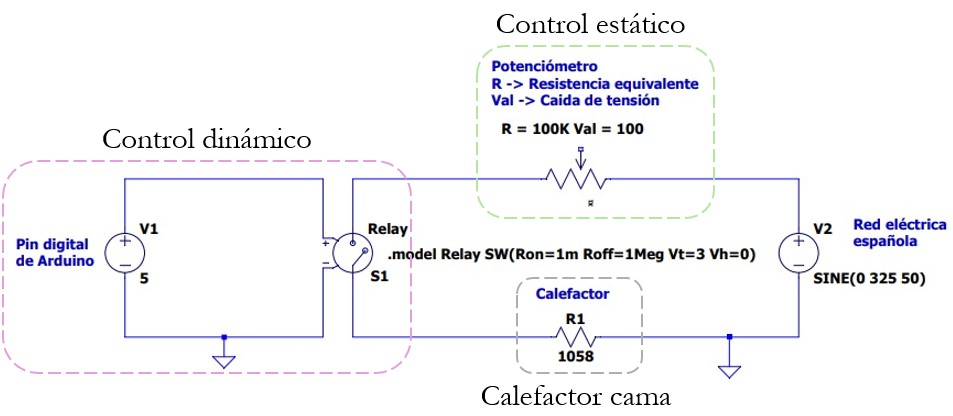
\includegraphics[scale=0.4]{figuras/Esquema electrico sistema regulacion termperatura.jpg}
    \caption{Sistema regulador de temperatura}
    \label{fig: Esquema eléctrico regulador de temperatura}
\end{figure}

\subsubsection*{Control estático}
\hypertarget{Control estático}{}
\bookmark[level=subsubsection,dest=Control estático]{Control estático}
La etapa de control estático es la responsable de proporcionar la tensión y corriente necesarias para que el cartucho calefactor comienza a calentarse por efecto Joule. El diseño eléctrico consiste en un potenciómetro de 100 K$\Omega$ de resistencia de referencia ubicado aguas abajo de la fuente de tensión proporcionada por la red eléctrica española. El diseño físico del potenciómetro utilizado es una rueda con un margen de giro 0-300º. 

La relación entre el ángulo de giro y el valor de la potencia eléctrica aportada no es lineal, motivo por el que teniendo en cuenta una temperatura objetivo de la cama de impresión de 60 ºC se calibró según la ecuación \ref{eq: linealizacion potenciometro}. En dicha expresión $P$ representa la potencia eléctrica suministrada al cartucho calefactor mientras que $x$ hace referencia al porcentaje de giro del potenciómetro sobre el total de 300º. El proceder técnico de esta tarea quedó a cargo de Irene Rodríguez, mientras que la revisión y corrección de cálculos fue responsabilidad del autor del trabajo.

\begin{equation}
\label{eq: linealizacion potenciometro}
    P(x)= 0,01234 + 0,01639x + 0,005208x^2
\end{equation}

\subsubsection*{Control dinámico}
\hypertarget{Control dinámico}{}
\bookmark[level=subsubsection,dest=Control dinámico]{Control dinámico}

La etapa de control dinámico es la responsable de regular la temperatura alcanzada por la cama de impresión en cada momento. Valora automáticamente si es necesario aportar más corriente para alcanzar el valor objetivo, gestiona que una vez alcanzado dicho valor se mantenga dentro de unos límites de seguridad y establece el procedimiento de actuación en caso de sobre calentamiento de la cama de impresión.

El equipo hardware se basa en el empleo de un microcontrolador con capacidad para registrar los datos de temperatura provenientes de la lectura del termopar, valorar el estado de la plataforma de impresión y comunicar su situación al resto de la estación. Esto es, la unidad de control conectada al computador central de la estación a través de comunicación serial.

El sistema implementa como acción controladora la conmutación de un relé ubicado aguas abajo de la etapa de control estático. La función principal del relé es permitir el paso de corriente hacia el cartucho calefactor, ajustando los tiempos de calentamiento y accionamiento de acuerdo con las simulaciones térmicas llevadas a cabo por Iñaki Echepare e Irene Rodríguez en sus respectivos trabajos. 

El ensayo térmico de un primer modelo que únicamente incluya la acción reguladora del relé variando entre los estados de encendido y apagado fue responsabilidad de Irene Rodríguez. También se llevaron sucesivos ensayos en los que se introducían otras acciones adicionales de control como el ajuste del periodo de conmutación o el envío de diferentes mensajes en función de la temperatura media alcanzada. Se valoró la inserción de un bloque regulador PID. Sin embargo, esta alternativa acabó descartándose ante la falta de componentes electrónicos comerciales que facilitasen a través del microprocesador el control de la intensidad eléctrica.

El algoritmo \ref{alg:algoritmo control dinámico de temperatura} muestra el funcionamiento del código desarrollado\footnote{Disponible en el repositorio de este proyecto y en el de Irene Rodríguez\cite{repo_github_Irene_Rodriguez}} para esta etapa de control. Se basa en la asignación durante el arranque de la plataforma de un valor de temperatura objetivo -llamado \textit{consigna}- que se evalúa constantemente con la información proveniente del termopar. La consigna es el valor enviado por el operario a través del canal que parte del computador central y pasa a la unidad de control. Cuando la unidad de control registra el valor de la consigna, el calentamiento de la cama arranca. La información que se utiliza para la gestión dinámica de temperatura de la cama es el promedio de temperatura de un conjunto de 10 medidas (la actual más las nueve anteriores), si ésta entra dentro del rango válido para la consigna se envía un mensaje indicando una correcta situación y se mantiene el relé encendido. Dada la evolución más lenta de los sistemas térmicos, se opta por establecer una frecuencia de muestreo de 0.5 Hz.

\begin{algorithm}[h!]
\caption{Control dinámico de temperatura}\label{alg:algoritmo control dinámico de temperatura}
\begin{algorithmic}[1]
\Require Temperatura consigna.
\Ensure Acción de control dinámico con apertura y cierre del relé.

\State Habilitar Señal Relé ON

\State Registrar temperatura consigna
\State Establecer rango válido de temperatura consigna. Límites superior e inferior.

\For{i $<$ 10}
    \State Leer temperatura instantánea de cama de impresión.
    \State Asignar temperatura leída a vector de comparación.
    \State Esperar dos segundos.
\EndFor

\While{No se indica fin de proceso de fabricación}
\State Efectuar promedio de vector de comparación.
\If{Temperatura promedio $<$ (Rango inferior consigna)}
    \State Señal Relé ON.
    \State Estado: CALENTANDO.
\EndIf
\If{Temperatura promedio $>$ (Rango superior consigna)}
    \State Señal Relé OFF.
    \State Estado: SOBRECALENTAMIENTO.
\EndIf
\If{(Temperatura promedio $>$ Rango inferior consigna) \textbf{y} (Temperatura promedio $<$ Rango superior consigna)}
    \State Señal Relé ON.
    \State Estado: TEMPERATURA EN RANGO.
\EndIf

\State Registrar temperatura actual en vector de comparación.
\State Esperar dos segundos.
\EndWhile
\end{algorithmic}
\end{algorithm}

El código representado por el anterior algoritmo ha sido desarrollado por Irene Rodríguez en colaboración con el autor de este proyecto, que ha llevado una labor de revisión del código, mantenimiento y valoración del comportamiento del sistema. Este código se integra dentro de un esquema que se sirve del uso de ROS2 para establecer una serie de hilos de comunicaciones entre la plataforma de impresión -mediante la unidad de control- y el computador central.

\subsection{Comunicaciones con la estación}

Como parte final del desarrollo del sistema de control de temperatura, se integra dentro del modelo de arquitectura informática del resto de la estación. Este modelo basa su funcionamiento en el empleo de ROS2 como gestor de comunicaciones entre diferentes procesos.

Para la gestión de la plataforma de impresión se decide definir un modelo de suscriptor-publicador entre el computador central y la unidad de control de la plataforma de impresión. El modelo se implementa a través de un paquete de nodos de ROS2 diseñados específicamente para esta tarea que se denomina \textit{build\_platform}.

El funcionamiento del nodo \textit{serial\_reader} se describe a través del algoritmo  , siendo el proceso encargado de la interpretación de mensajes provenientes de la plataforma de impresión. Se trata de un sistema responsable del envío y lectura los siguientes mensajes:
\begin{itemize}
    \item \textbf{Arranque y apagado de la unidad de control:} Mensaje comandado desde el computador central en el que se indica el inicio del sistema de calentamiento de la cama de impresión. Para favorecer la modularidad del equipo, se decide que éste sea el único mensaje que se puede enviar hacia la plataforma de impresión. En otras palabras, se deja que el equipo servidor pueda gestionarse automáticamente.
    \item \textbf{Estado de la plataforma:} Mensaje generado por la unidad de control que comunica al computador central variables de interés como si el calefactor se encuentra encendido o no, el valor de la temperatura registrada en dicho instante o si está en aumento y descenso. Este mensaje se envía en formato de cadena de texto, dejando la responsabilidad de su interpretación al nodo ejecutándose en el computador central.
\end{itemize}

\begin{algorithm}[h!]
\caption{serial\_reader}\label{alg:algoritmo lectura estado plataforma de impresión}
\begin{algorithmic}[1]
\Require Valor de temperatura consigna.
\Ensure Registro continuo de estado de la plataforma de impresión.

\State Arrancar suscriptor a al puerto de comunicaciones con la plataforma de impresión.
\State Enviar valor de temperatura consigna a la unidad de control.
\State Confirmar recepción de temperatura consigna en unidad de control.

\While{No se cierra el nodo en ejecución}
\State Leer mensaje proveniente de la unidad de control.
\State Archivar valor medido
\State Archivar estado evaluado
\State Esperar 1 segundo
\EndWhile

\end{algorithmic}
\end{algorithm}


Como primera iteración se decide efectuar una comunicación entre el microcontrolador y el computador central a través de un puerto serie. Aprovechando la capacidad de paralelización de procesos que ofrece ROS2 a través de su estructura de nodos (de forma análoga al ejemplo descrito en la sección \ref{sec: ejemplo implementacion diseño arquitectura}), el algoritmo queda definido para que se pueda implementar en futuros proyectos con otros protocolos de comunicación de tipo \acrshort{TCP/IP} como puede ser MODBUS-RTU o MQTT.

Se especifica un total de cinco mensajes para informar del estado de la plataforma según una clave numérica, éstos son:
\begin{itemize}
    \item \textbf{Estado 0:} Regulador de temperatura encendido y cama calentándose. La temperatura promedio registrada es menor que el límite admisible inferior.
    \item \textbf{Estado 1:} Regulador de temperatura encendido y cama calentada. La temperatura promedio registrada se encuentra dentro de los límites programados para la consigna.
    \item \textbf{Estado 2:} Regulador de temperatura encendido y cama sobrecalentada. La temperatura promedio medida es mayor que el límite admisible superior. El proceso puede estar ejecutándose en condiciones no deseadas y se recomienda revisar su funcionamiento.
    \item \textbf{Estado 3:} Regulador de temperatura apagado y cama enfriándose. La temperatura promedio registrada es superior a 30 ºC.
    \item \textbf{Estado 4:} Regulador de temperatura apagado y cama enfriada. La temperatura promedio registrada es inferior a 30 ºC.
\end{itemize}


\section{Resultados y conclusiones}
En esta sección se procede a describir los resultados de los ensayos realizados comentando su ejecución y el comportamiento observado. Posteriormente se extraen una serie de valoraciones acerca de las ventajas e inconvenientes observados ante el modelo propuesto.

\subsection{Resultados}
Con los elementos definidos en la metodología del capítulo, se construye un prototipo del sistema que se ejecuta en un entorno seguro. En el momento de realización del ensayo, la plataforma de impresión no disponía de un encapsulamiento adecuado, por lo que el entorno de ensayo únicamente se compuso del prototipo electrónico de la plataforma de impresión y el computador central con el entorno de simulación ROS2. La Figura \ref{fig:montaje_termopar} muestra una fotografía del montaje experimental de este equipo y se señalan todos los componentes que componen la electrónica de control.

\begin{figure}[H]
    \centering
    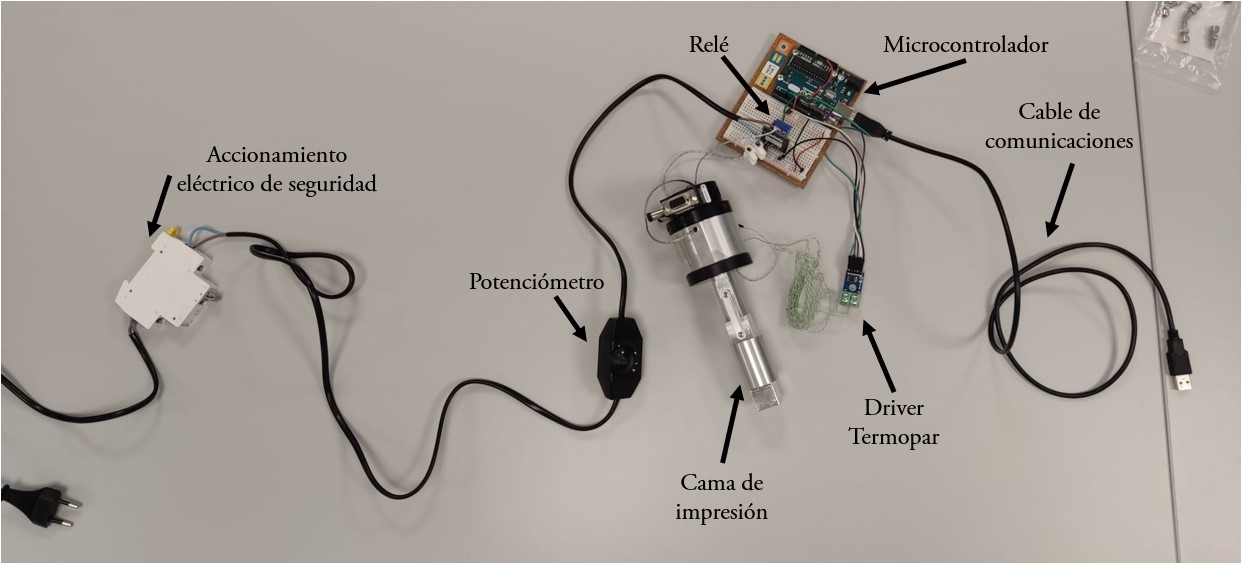
\includegraphics[scale=0.30]{figuras/montaje ensayo control temperatura.jpg}
    \caption{Montaje físico del sistema de control de temperatura}
    \label{fig:montaje_termopar}
\end{figure}

Se procede a conectar la plataforma de impresión a la red eléctrica y al computador central, decidiendo efectuar dos ensayos. El primero de ellos se hace con una carga de potencia reducida de valor objetivo de aproximadamente 6 W y una consigna de 40 ºC. En este ensayo se busca respetar la integridad de los componentes y validar la correcta comunicación entre la plataforma de impresión y el resto de la estación robotizada. Se prevé que en este ensayo no se pueda mantener el valor de la consigna en el tiempo al no disponer de la potencia de trabajo necesaria. 

El segundo realiza el calentamiento de la cama a la potencia de trabajo de 9.2 W y a una consigna de 60 ºC que es el valor deseado para la estación. El objetivo del ensayo es validar el correcto comportamiento del sistema de regulación de temperatura implementado. En este caso, al disponer de toda la potencia de trabajo proyectada se espera que se ejecute una regulación constante en torno al valor de la consigna, una vez llegue a él.

Los resultados del ensayo a 6 W se muestran en la Figura \ref{fig: Ensayo plataforma impresion 6 W lectura estado}. En ella se aprecia la correcta lectura de la temperatura en la terminal del computador central (Figura \ref{fig: lectura estado plataforma impresion}), información que sigue el esquema descrito en la Figura \ref{fig:arquitectura plataforma impresión} y proviene de un procesamiento previo de la unidad de control. Así mismo, la Figura \ref{fig: ensayo plataforma impresion 6 W} ilustra conceptualmente un registro de previo datos de temperatura realizado con la hoja de cálculo Excel. El registro se adecúa al comportamiento esperado ante una versión reducida en la que también se registra un periodo de enfriamiento comandado por el operario a partir de los 600 segundos.

\begin{figure}[H]
    \centering
     \begin{subfigure}[h]{0.45\linewidth} 
        \centering
        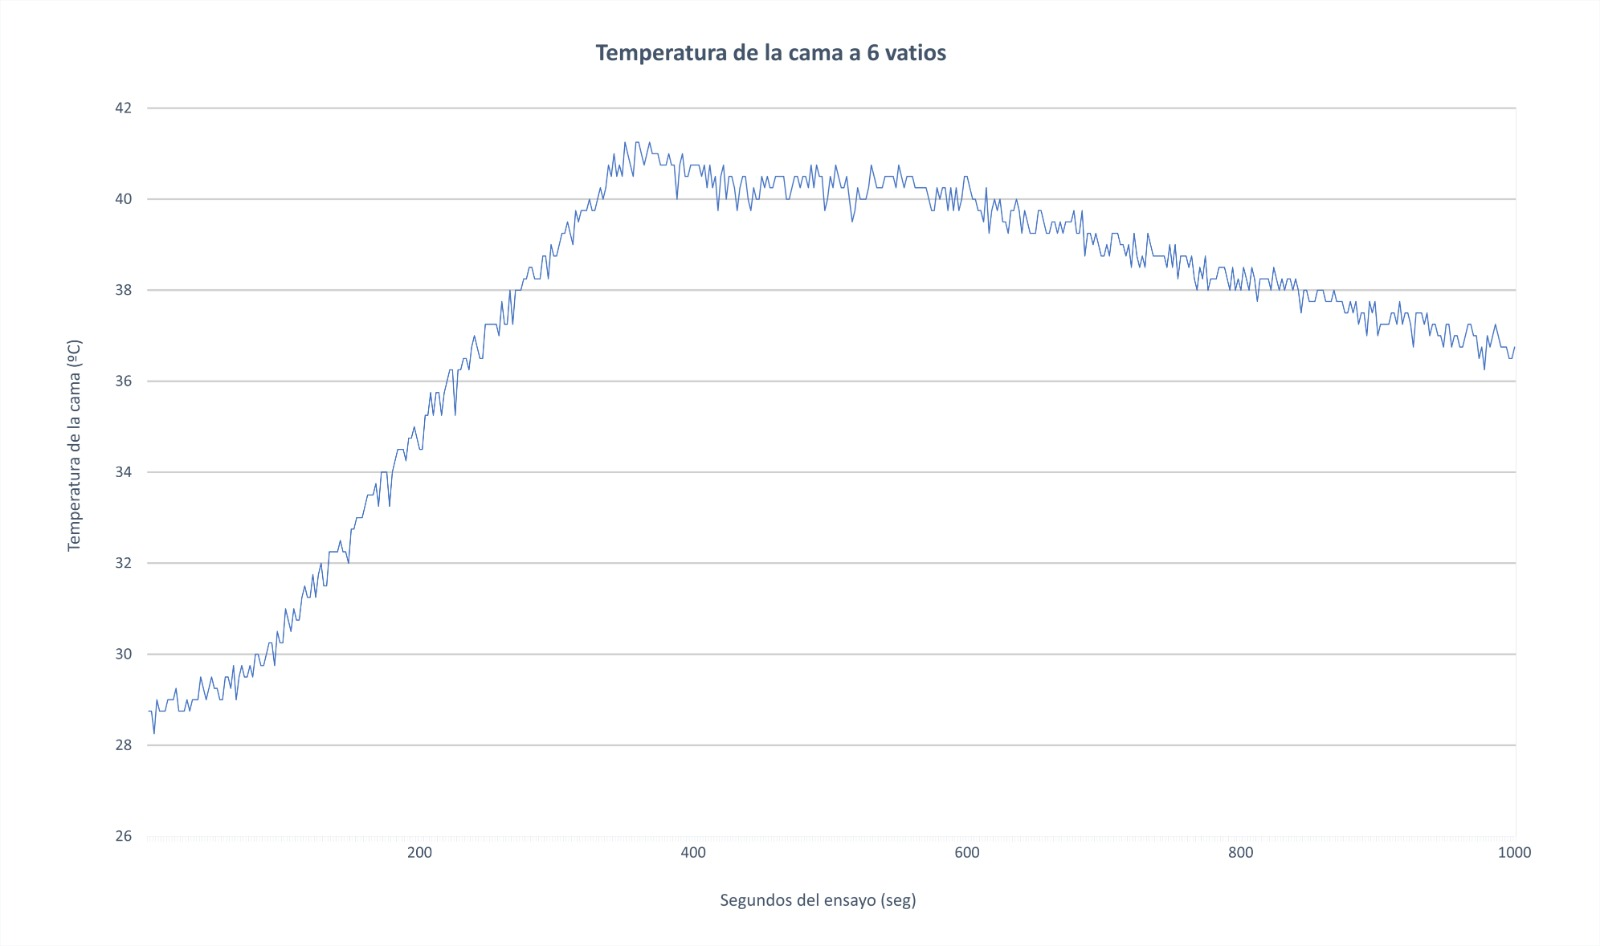
\includegraphics[scale=0.15]{figuras/ensayo plataforma impresion 6 W.jpeg}
        \caption{Temperatura registrada}
        \label{fig: ensayo plataforma impresion 6 W}
    \end{subfigure}
    \begin{subfigure}[h]{0.45\linewidth} 
        \centering
        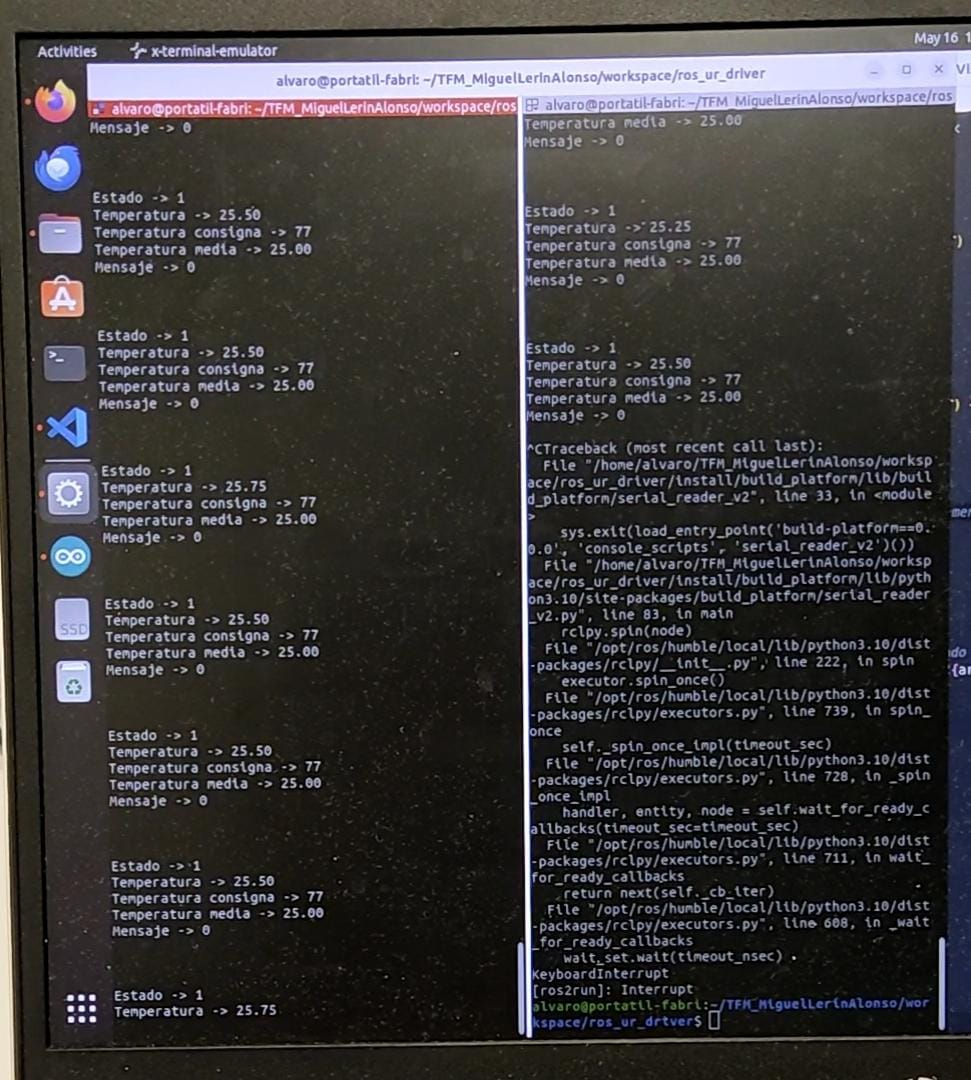
\includegraphics[scale=0.14]{figuras/lectura estado plataforma impresion.jpeg}
        \caption{Lectura de estado de la plataforma de impresión}
        \label{fig: lectura estado plataforma impresion}
    \end{subfigure}
    \caption{Ensayo de 6 W. Comunicación plataforma-estación}
    \label{fig: Ensayo plataforma impresion 6 W lectura estado}
\end{figure}

Por parte del ensayo de 9 W de la Figura \ref{fig: Ensayo plataforma impresion 9 W}, se observa que al disponer de la totalidad de la potencia de trabajo la acción de control puede mantenerse indefinidamente en el tiempo. 

\begin{figure}[H]
    \centering
    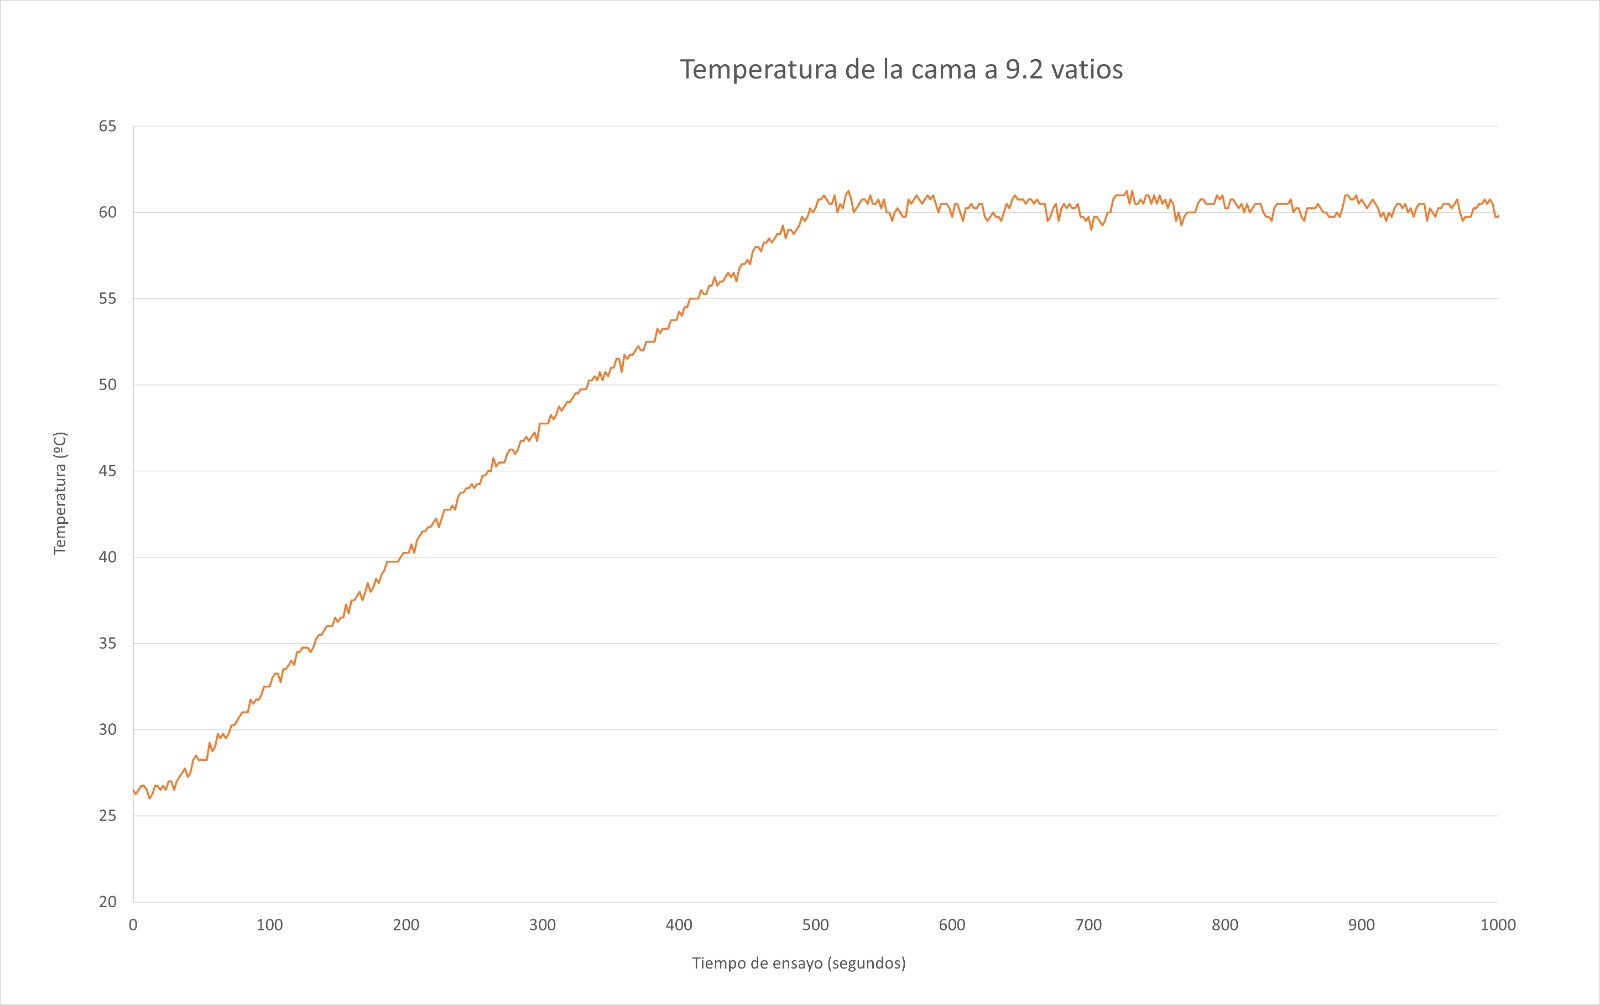
\includegraphics[scale=0.15]{figuras/Ensayo plataforma impresion 9 W.jpeg}
    \caption{Ensayo de 9 W. Regulación de temperatura}
    \label{fig: Ensayo plataforma impresion 9 W}
\end{figure}

Cabe destacar que, al igual que en el ensayo anterior, el incremento de temperatura se da de forma lineal con el tiempo transcurrido. En este caso, la mayor cantidad de potencia de entrada favorece que se alcance el valor de la consigna en un menor tiempo, con una pendiente de aproximadamente 4.67 ºC/min frente a los 1.33 ºC/min. 

\subsection{Conclusiones}
El modelo de plataforma de impresión propuesto ofrece varias ventajas al funcionamiento global de la estación, como su facilidad de uso, capacidad modular y gestión a través de la interfaz proporcionada por ROS2. Aunque no se han podido realizar ensayos con la plataforma de impresión finalizada, los resultados indican que se trata de un equipo robusto y altamente flexible.

Diversos aspectos facilitan el uso de la plataforma de impresión como un elemento escalable para su implementación en otros procesos de fabricación aditiva. Por un lado, la capacidad de tratar la plataforma de impresión como un módulo independiente de otros procesos de la estación favorece una gestión autónoma del sistema de calentamiento. Esto permite enfocarse en labores de ingeniería de diseño mecánico y de producto especializadas en la cama de impresión y los elementos disipadores de calor que integra. Por otro lado, la arquitectura de control implementada permite aislar la alimentación del sistema del control de temperatura. De modo que se deja la calibración del primero como responsabilidad del operario para cada producto a fabricar y el segundo como una gestión automática realizada por la unidad de control.

Finalmente, la integración de una arquitectura de comunicaciones propia basada en ROS2 favorece la interacción de la plataforma con el resto de la estación. Se define un estándar común de comunicaciones que permite al ingeniero responsable evaluar el desempeño de cada equipo sin interrumpir el flujo de trabajo. También permite introducir desde un nivel de abstracción superior nuevos mensajes y estados de emergencia que pueden configurarse rápidamente entre ambos dispositivos.

\begin{figure}[h!]
    \centering
    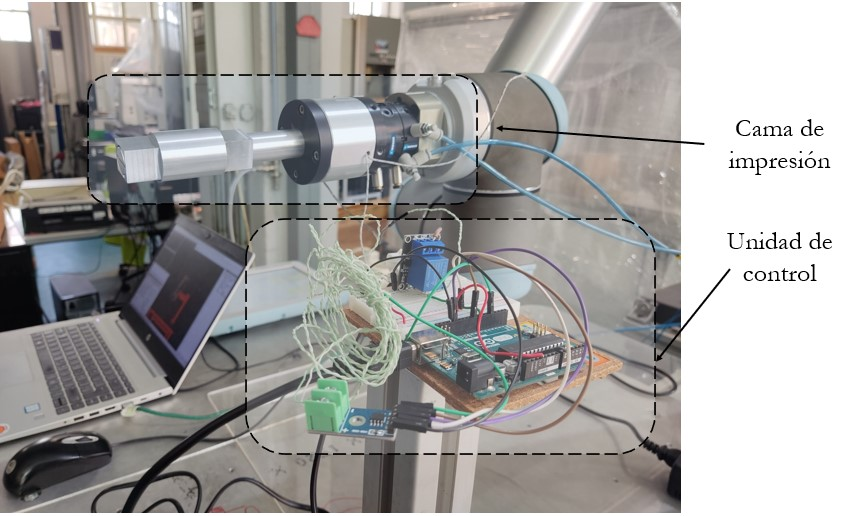
\includegraphics[scale=0.43]{figuras/Montaje prototipo cama impresion.jpg}
    \caption{Montaje de prototipo de plataforma de impresión}
    \label{fig: montaje prototipo plataforma de impresión}
\end{figure}

No obstante, la plataforma de impresión presenta desafíos adicionales y se encuentra en un estado que alcanza los límites del proyecto. Se ha logrado diseñar, implementar y validar un modelo de arquitectura de control que (1) se comunica con el resto de los elementos de la estación y (2) gestiona automáticamente su propio proceso de calentamiento. Sin embargo, aún quedan pendientes tareas relacionadas con la optimización del sistema de evacuación de calor de la cama, el diseño de un encapsulamiento protector del hardware y la fabricación de un microcontrolador específico para esta arquitectura. Estas tareas se abordarán en otros trabajos como el de Irene Rodríguez.

Como muestra del estado actual de la plataforma, se presenta la Figura \ref{fig: montaje prototipo plataforma de impresión}. En ella se aprecia la integración parcial de la plataforma con el resto de los componentes de la estación, como el computador central y el manipulador robótico. Sobre el soporte ubicado al lado de la cama de impresión, se observa el prototipo de hardware realizado para la unidad de control.

